%!TEX root = ../dokumentation.tex
\chapter{Continuous Integration}\label{ch:continuous-integration}

Um das in der Vorlesung behandelte Thema der CI/CD-Pipeline zu behandeln, wurde in diesem Projekt die freie und Open-Source-Software Travis-CI verwendet. Die Software wurde zuvor in anderen Projekten erfolgreich verwendet, weshalb die Nutzung von Tools wie Azure Pipelines, Jenkins oder TeamCity nicht in Betracht gezogen wurde.
Zur Konfiguration der CI/CD-Software wurde bei \hyperlink{https://travis-ci.com/}{Travis-CI} das GitHub Repository dieses Projekts hinterlegt. Travis-CI generiert für jeden neuen Commit auf dem Master-Branch des Repositories einen Build. Bei der Erzeugung des Builds wird geprüft, ob die Docker Container mit den darin enthaltenen Backend/Frontend Lösungen fehlerfrei starten. Hierfür sind die folgenden Konfigurationen festgelegt worden.

\begin{figure}[H]
 \centering
 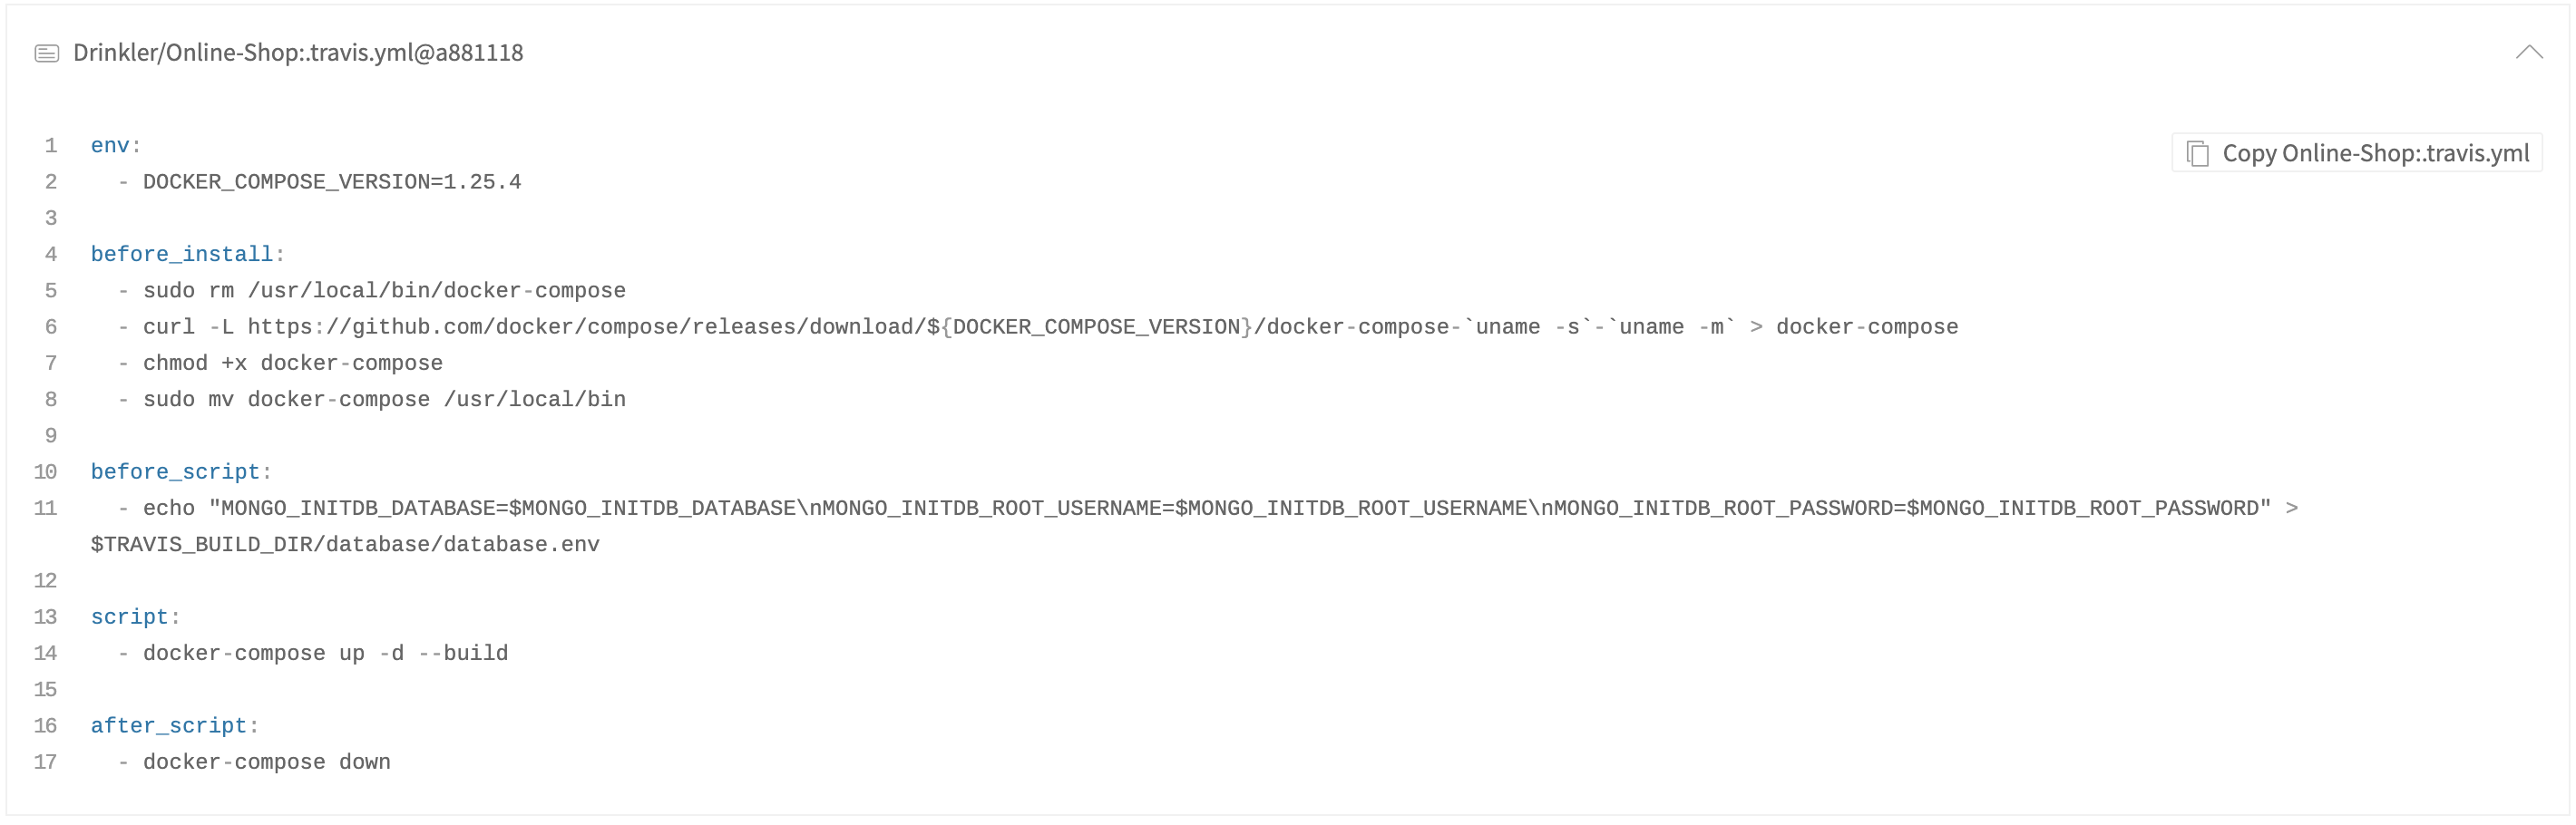
\includegraphics[width=\textwidth,height=0.6\textheight,keepaspectratio]{images/Travis-CI-conf.png}
 \caption{Travis-CI Konfiguration}
 \label{fig:ci-conf}
\end{figure}

\begin{figure}[h]
 \centering
 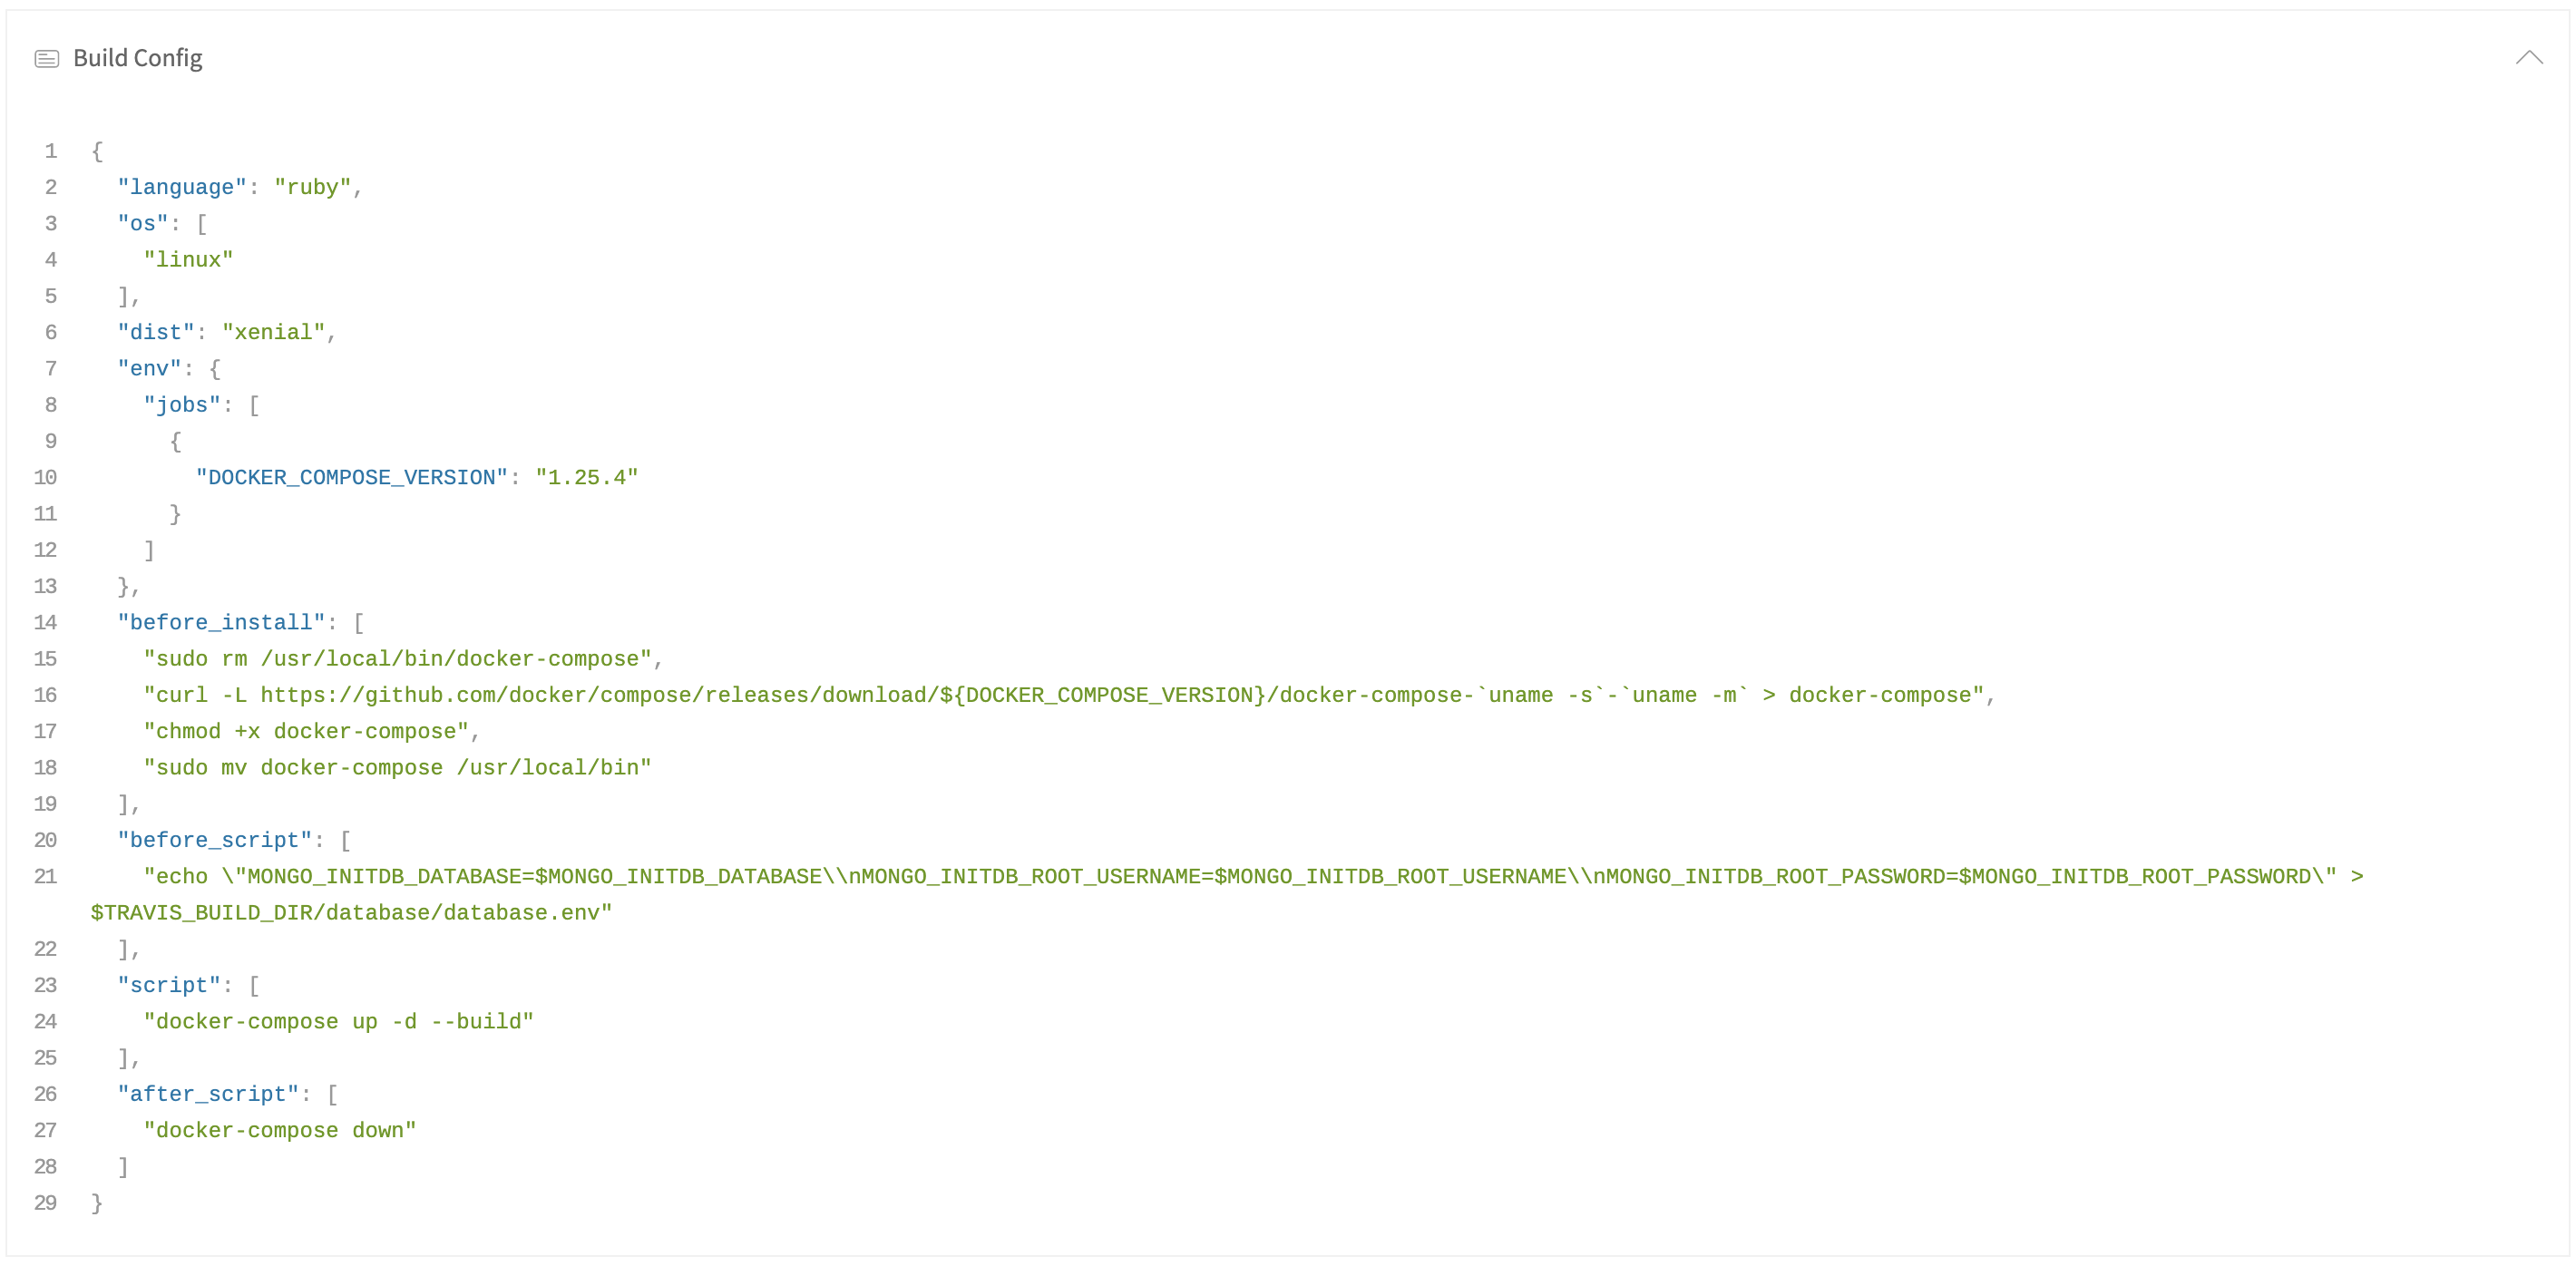
\includegraphics[width=\textwidth,height=0.6\textheight,keepaspectratio]{images/Build-conf.png}
 \caption{Travis-CI Build-Konfiguration}
 \label{fig:build-conf}
\end{figure}
